\section{实验:安装简单的照明电路}\label{sec:11-5}

要掌握照明电路的安装、检修技能,必须经过专门的训练,严格遵照操作规程反复实践,
绝不是在物理实验室里练习一次就能掌握的。
但是在学过照明电路的简单知识以后,在木板上练习安装图 \ref{fig:11-11} 所示的简单照明电路,
对于巩固我们学得的知识和初步了解一些安装方法还是有好处的。

\begin{figure}[htbp]
    \centering
    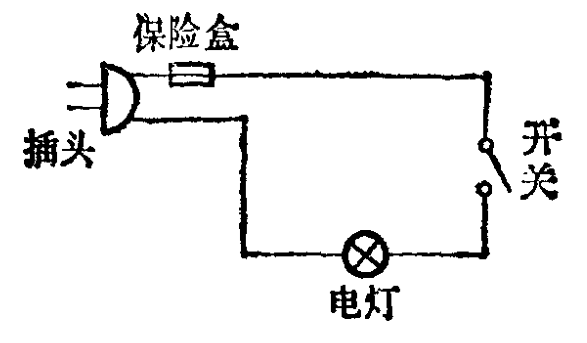
\includegraphics[width=0.5\textwidth]{../pic/czwl2-ch11-11}
    \caption{在木板上安装的简单照明电路示意图}\label{fig:11-11}
\end{figure}

即使是安装简单的照明电路,也应该先作个计划。计划的内容包括:
(1) 确定灯座、开关等设备的安装位置和电线的敷设路径;
(2) 列出需用的器材的规格和数量;
(3) 安排好安装的步骤。
计划不一定要写出来,但必须心中有数。
我们是在木板上安装, 老师已经给准备好了器材,只要明确安装步骤就可以了。
步骤大致是:标划电线、设备的安装位置,装上固定电线的瓷夹板,敷设电线,
装上各种电气设备,检查电路,接通电源。

安装照明电路的时候,必须把电灯的开关接在火线上,这样,拉开开关切断电路时,
灯座脱离火线,人碰到灯座不会触电。
螺丝口灯座的螺旋套则只准接在零线上,不准接在火线上(想一想为什么)。

在木板上安装的时候,可以先确定某一条电线将来接到电源的火线上,再按照下面的口诀敷设电线:

\vspace{-1em}
\begin{center}
    火线零线并排走,\qquad 零线直接进灯座;

    火线接进保险盒,\qquad 再过开关进灯座。
\end{center}

\vspace{-1em}
要认真学习连接导线以及安装灯座、开关、插头、保险盒、保险丝的正确方法,
严格按照技术要求去操作,把电路安装得牢靠, 整齐。

装好后要检查有没有短路、断路,并且记清插头的哪个插脚应当连接火线。
请老师复查以后装上电灯泡。

用测电笔判定电源插座的哪个孔连着火线。
然后在老师监督下,将插头插入电源插座。
闭合开关,看电灯是否发光。

如果实验用的开关是拉线开关,在电路装好、电灯正常发光以后如果还有时间,
可以拨下插头,切断电源,拧下开关的盖,看看开关中的拉线是怎样穿着的。
然后拉动拉线,观察开关怎样通、断电路。



\lianxi

(1) 为了用电安全,为什么必须注意下面几点?

\tc{1} 不准用剪刀或没有绝缘柄的钳子剪带电的导线;

\tc{2} 不准在电线上晾衣服;

\tc{3} 发现有人触电时,必须先切断电源;然后才可以直接用手去拉他;

\tc{4} 发现输电线的断头落在地上,不要走近,更不准去拾。

(2) 图 \ref{fig:11-12} 中所示的几个螺丝口灯座的连接,哪个对,哪个错?错在哪里?

\begin{figure}[H]%[htbp]
    \centering
    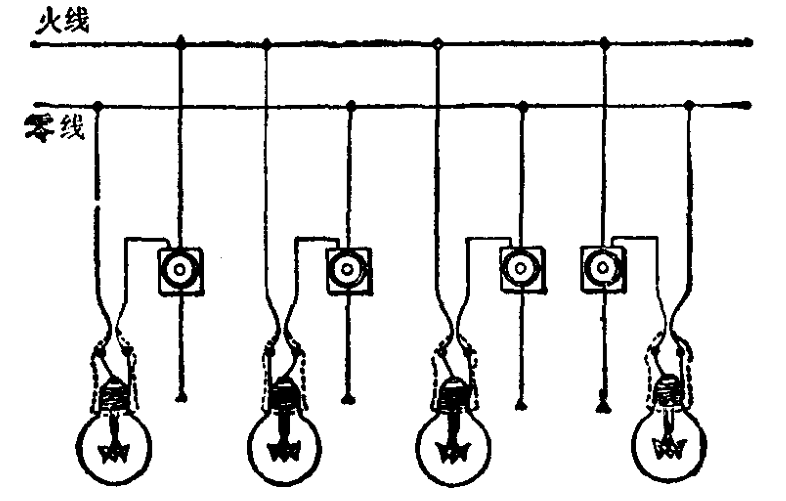
\includegraphics[width=0.8\textwidth]{../pic/czwl2-ch11-12}
    \caption{}\label{fig:11-12}
\end{figure}

(3) 插座,特别是准备接大功率用电器的插座,常常要在通插座的火线上装一根保险丝,
而不是在通插座的火线和零线上各装一根保险丝。
这样作不是为了省一根保险丝,而是为了更安全。想想看,为什么这样更安全?



\section*{小实验}

\begin{figure}[htbp]
    \centering
    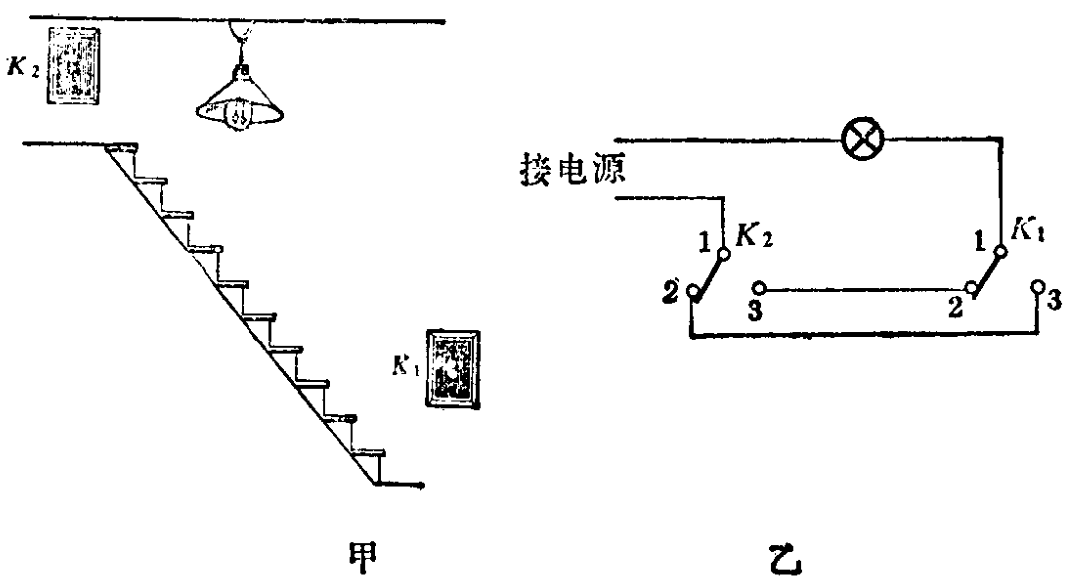
\includegraphics[width=0.9\textwidth]{../pic/czwl2-ch11-13}
    \caption{}\label{fig:11-13}
\end{figure}

在楼梯(或楼道)中间安装的电灯,需要在楼梯的上、下两头都能控制它(图 \ref{fig:11-13} 甲):
当上楼梯时,能用下面的开关 $K_1$ 开灯,人上了楼梯以后, 能用上面的开关 $K_2$ 关灯;
当下楼梯时,能用 $K_2$ 开灯,用 $K_1$ 关灯。
图 \ref{fig:11-13} 乙是用两个单刀双掷开关控制一盏灯的电路图。
单刀双掷开关的掷刀可以绕轴 1 转动,或者跟触头 2 接触或者跟触头 3 接触。
分析一下 $K_1$、$K_2$ 中的任何一个都能开灯、关灯的道理。
按照图 \ref{fig:11-13} 乙所示的电路图,在木板上用电池、小灯泡、两个单刀双掷开关组成电路,
并且试验这个电路中的两个开关是不是都能开灯、关灯。
如果没有单刀双掷开关,可以采取代替的办法,
例如在木板上按三个图钉分别代替轴 1 和触头2、3,
用一段铜线代替掷刀,接在1、2 间,或者接在1、3 间。

